% 2012 辽宁文 20 题图：椭圆 C2: x^2/9+y^2=1 与动圆 C1: x^2+y^2=t^2 交于 A,B,C,D，
% A1,A2 为椭圆左右顶点；取代表值 t=1.8（1<t<3，schematic）。
\usetikzlibrary{arrows.meta,calc}
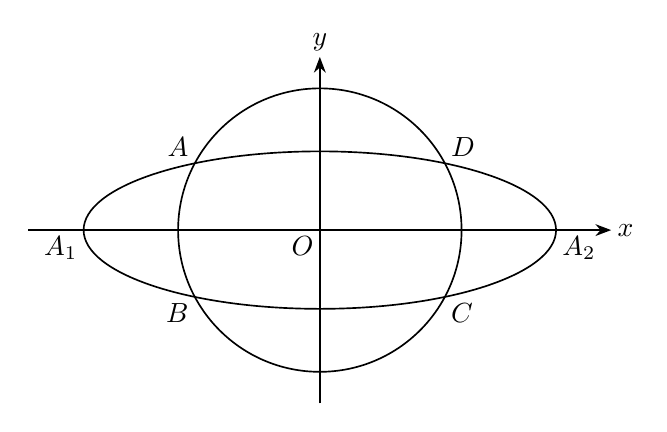
\begin{tikzpicture}[x=1cm,y=1cm,line width=.6pt,>=Stealth,font=\normalsize]
\draw[->] (-3.7,0)--(3.7,0) node[right,inner sep=2pt]{$x$};
\draw[->] (0,-2.2)--(0,2.2) node[above,inner sep=2pt]{$y$};
\draw (0,0) ellipse [x radius=3, y radius=1];
\draw (0,0) circle [radius=1.8];
\coordinate (A)  at (-1.5874508,0.8485281);
\coordinate (D)  at (1.5874508,0.8485281);
\coordinate (B)  at (-1.5874508,-0.8485281);
\coordinate (C)  at (1.5874508,-0.8485281);
\coordinate (A1) at (-3,0);
\coordinate (A2) at (3,0);
\node[above left,inner sep=2pt] at (A) {$A$};
\node[above right,inner sep=2pt] at (D) {$D$};
\node[below left,inner sep=2pt] at (B) {$B$};
\node[below right,inner sep=2pt] at (C) {$C$};
\node[below left,inner sep=2pt] at (A1) {$A_1$};
\node[below right,inner sep=2pt] at (A2) {$A_2$};
\node[below left,inner sep=2pt] at (0,0) {$O$};
\end{tikzpicture}
